\documentclass[tikz,border=10pt]{standalone}
\usepackage{tikz}
\usetikzlibrary{arrows.meta,positioning,calc,shapes.geometric}

\begin{document}
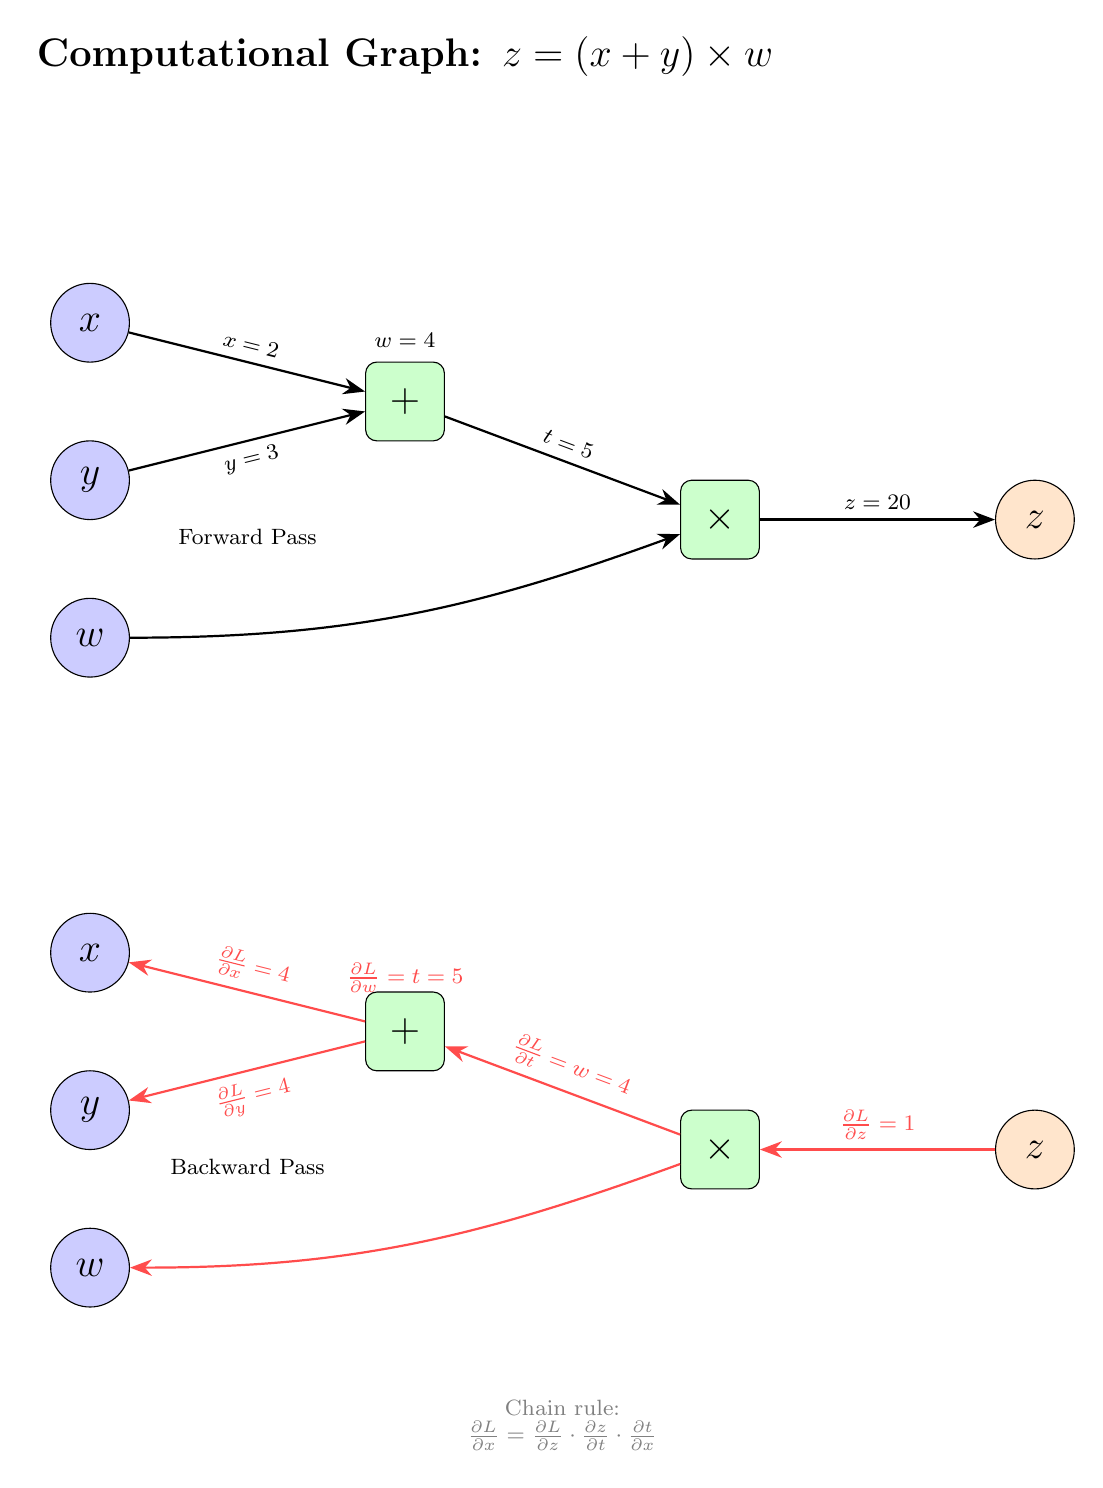
\begin{tikzpicture}[
    node distance=2.5cm,
    every node/.style={font=\sffamily},
    input/.style={circle, draw, fill=blue!20, minimum size=1cm, font=\Large},
    operation/.style={rectangle, draw, fill=green!20, minimum size=1cm, rounded corners, font=\Large},
    output/.style={circle, draw, fill=orange!20, minimum size=1cm, font=\Large},
    arrow/.style={-{Stealth[scale=1.2]}, thick},
    gradient/.style={-{Stealth[scale=1.2]}, thick, red!70},
    label/.style={font=\footnotesize, text centered}
]

% Title
\node[above=3cm, font=\Large\bfseries] at (0,0) {Computational Graph: $z = (x + y) \times w$};

% Forward pass section
\node[label, below=2.5cm] at (-2,0) {Forward Pass};

% Input nodes
\node[input] (x) at (-4, 0) {$x$};
\node[input] (y) at (-4, -2) {$y$};
\node[input] (w) at (-4, -4) {$w$};

% Operation nodes
\node[operation] (add) at (0, -1) {$+$};
\node[operation] (mul) at (4, -2.5) {$\times$};

% Output
\node[output] (z) at (8, -2.5) {$z$};

% Forward edges
\draw[arrow] (x) -- (add) node[midway, above, sloped, label] {$x=2$};
\draw[arrow] (y) -- (add) node[midway, below, sloped, label] {$y=3$};
\draw[arrow] (add) -- (mul) node[midway, above, sloped, label] {$t=5$};
\draw[arrow] (w) to[out=0,in=200] (mul) node[midway, below, sloped, label] {$w=4$};
\draw[arrow] (mul) -- (z) node[midway, above, label] {$z=20$};

% Backward pass section (below)
\begin{scope}[yshift=-8cm]
\node[label, below=2.5cm] at (-2,0) {Backward Pass};

% Same structure for backward
\node[input] (x2) at (-4, 0) {$x$};
\node[input] (y2) at (-4, -2) {$y$};
\node[input] (w2) at (-4, -4) {$w$};
\node[operation] (add2) at (0, -1) {$+$};
\node[operation] (mul2) at (4, -2.5) {$\times$};
\node[output] (z2) at (8, -2.5) {$z$};

% Gradient flow (backward)
\draw[gradient] (z2) -- (mul2) node[midway, above, label] {$\frac{\partial L}{\partial z} = 1$};
\draw[gradient] (mul2) -- (add2) node[midway, above, sloped, label] {$\frac{\partial L}{\partial t} = w = 4$};
\draw[gradient] (mul2) to[out=200,in=0] (w2) node[midway, below, sloped, label] {$\frac{\partial L}{\partial w} = t = 5$};
\draw[gradient] (add2) -- (x2) node[midway, above, sloped, label] {$\frac{\partial L}{\partial x} = 4$};
\draw[gradient] (add2) -- (y2) node[midway, below, sloped, label] {$\frac{\partial L}{\partial y} = 4$};

% Annotations
\node[label, text=gray, align=center] at (2, -6) {Chain rule:\\$\frac{\partial L}{\partial x} = \frac{\partial L}{\partial z} \cdot \frac{\partial z}{\partial t} \cdot \frac{\partial t}{\partial x}$};
\end{scope}

\end{tikzpicture}
\end{document}